\section{Evaluation}

Three studies were conducted to answer new research questions or rephrase existing ones. These studies are grouped into 2 phases, and each tested a different version of \chameleon{} with human participants. The number of participants and their Haskell experience, as well as key research questions and conclusions, were shown in figure \ref{fig:timeline}. \todo{Explain was a user study of the tool with practitioners?}


\begin{figure*}
    \centering
    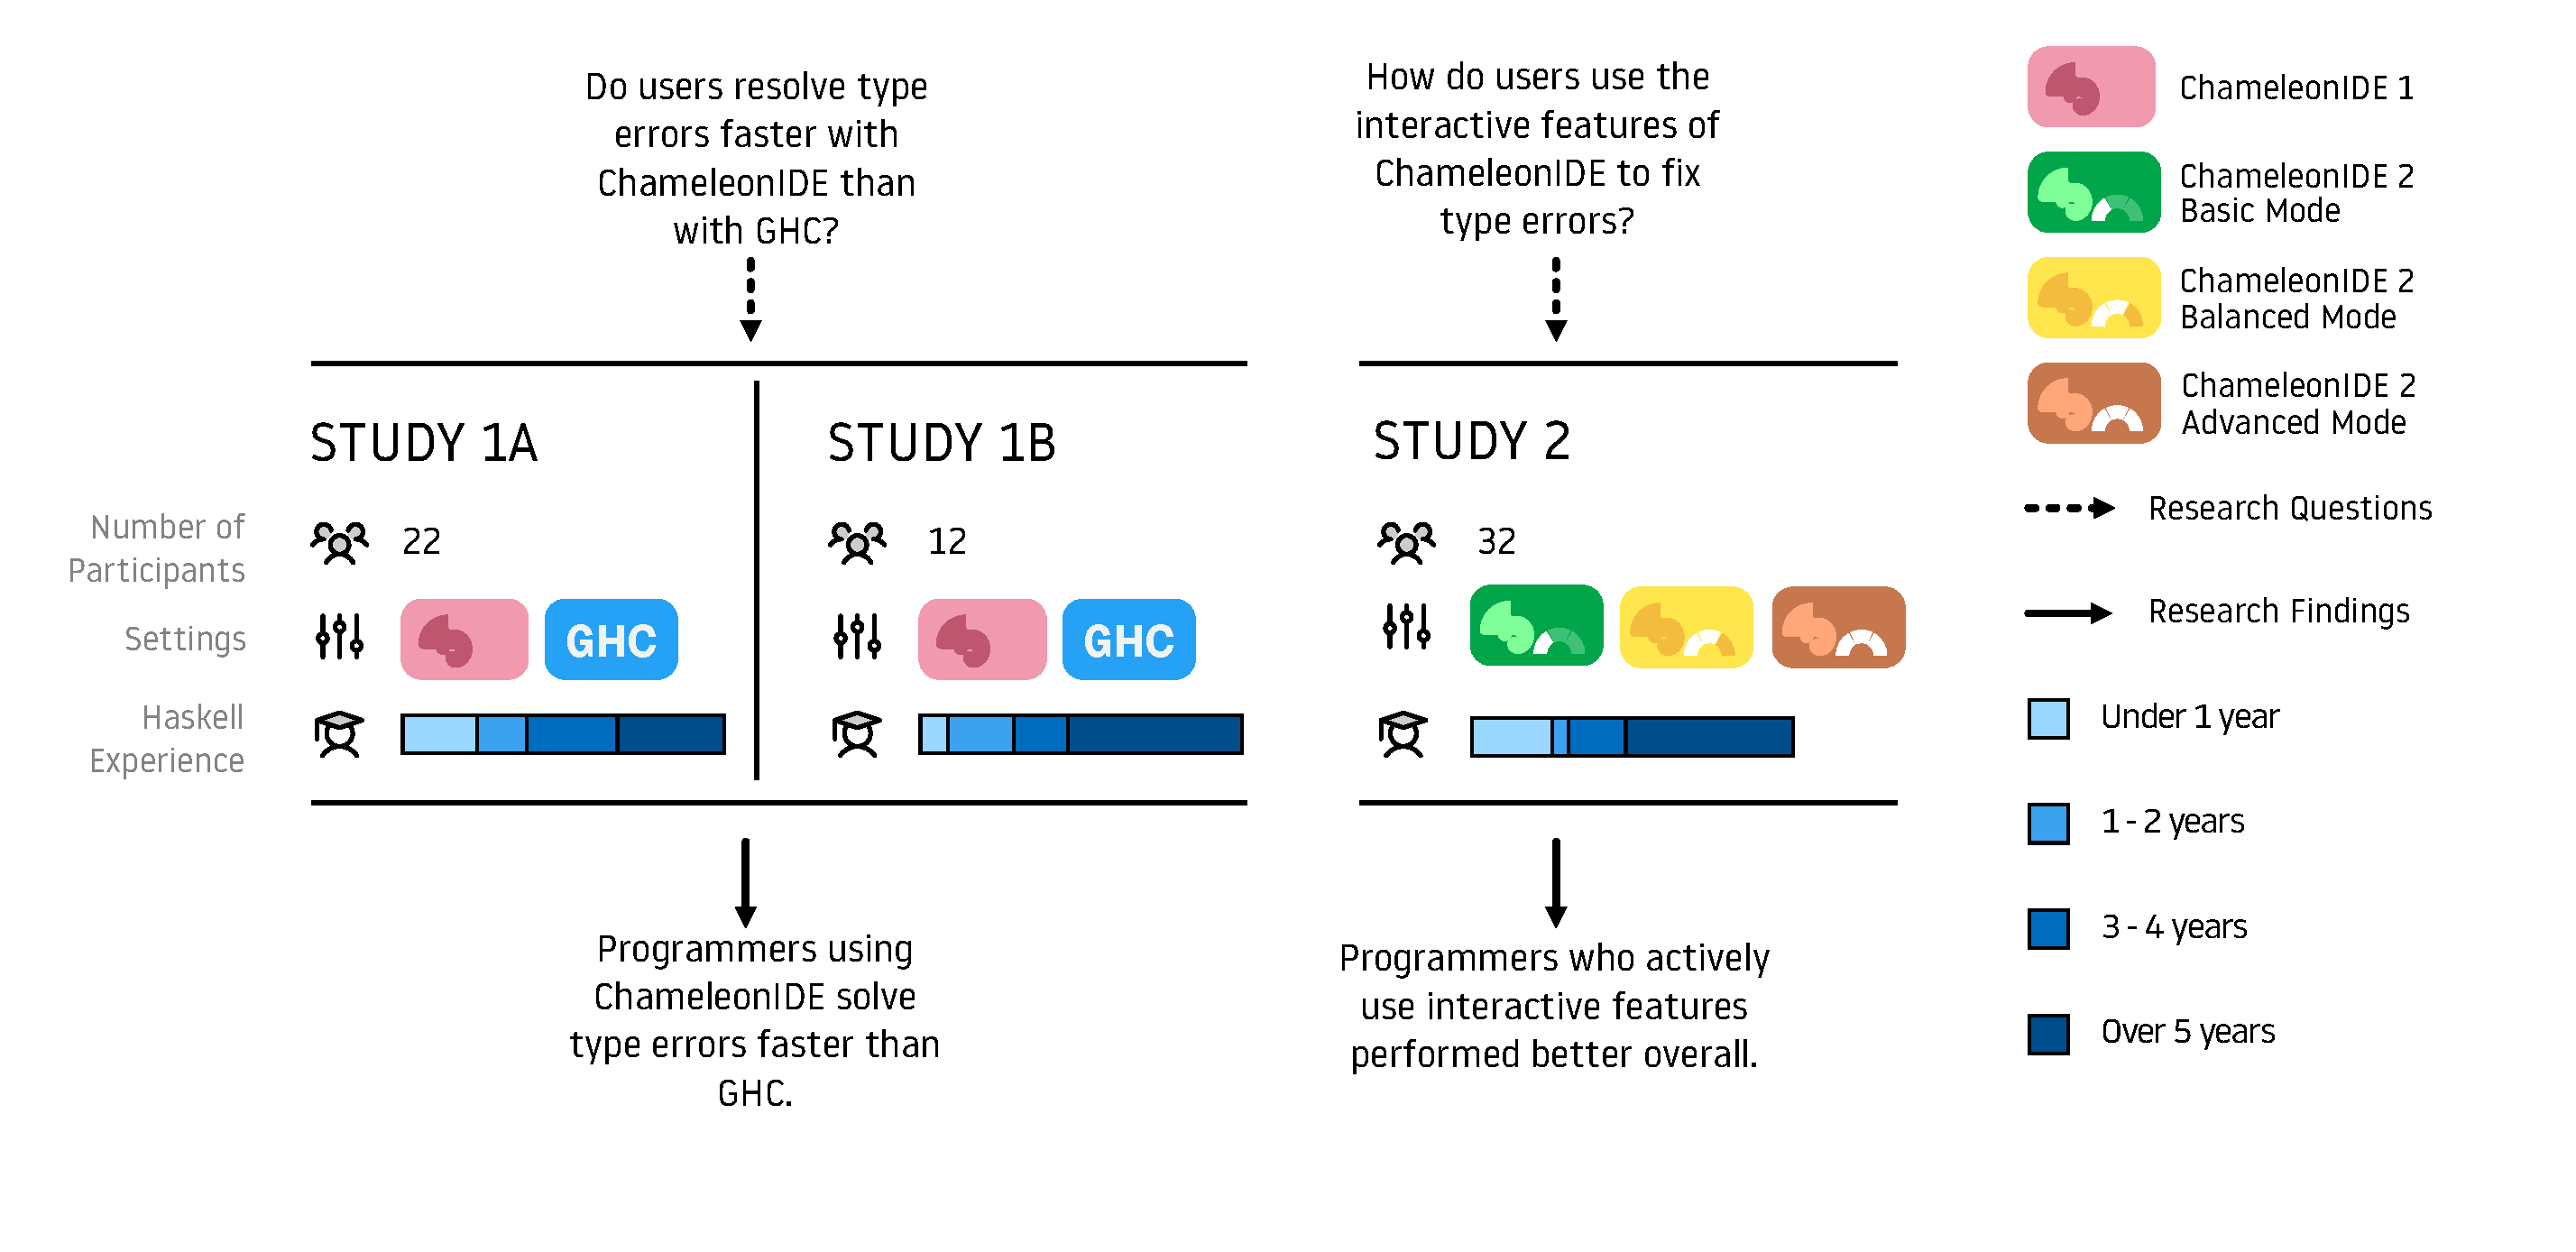
\includegraphics[width=\textwidth]{images/timeline.pdf}
    \caption{The timeline of \chameleon{}  evaluation.}
    \label{fig:timeline}
\end{figure*}

\subsection{Experiment Design}
\subsubsection*{\textbf{Recruitment}}

The recruiting channel we used was the social news aggregation website Reddit. Specifically, our user study advertisements were posted in the Haskell programming language community \textit{r/haskell} and a general "programming language" focused community \textit{r/programminglanguages}. Recruiting from social media allowed us to access a more diverse demographic that better represent the true population of Haskell programmers. The participation is fully anonymized. The detailed ethical implications of these experiments are reviewed and approved by the IRB of the institution of the authors.

\todo{Need more detail on participants - years experience, male vs female, etc}


\subsubsection*{\textbf{Experiment setting}}
The experiments took place remotely and unsupervised. Participants took the study online via a web browser and at the physical venue of their choosing. All user studies use a web-based debugging environment developed by the authors. Conducting the studies online helped us avoid variation when performing tasks in unfamiliar places and using different setups. 


\subsubsection*{\textbf{Training and group assignment}}
After consent, participants received interactive training on the tool interface and interactive features. Participants were also shown a cheat sheet summarizing the key functionality of the interface. Participants had access to the cheat sheet at all times during the study. Participants were given 4 trial runs (2 for each setting) before the data collection started. 

All the user studies used a within-subject design to evaluate the effectiveness of different tools or feature sets while counterbalancing the difference in programming proficiency between participants. In each study, participants were required to complete a series of programming tasks (8 for studies 1a and 1b, 9 for study 2). At each task, a participant receives a single Haskell file that contains one or more type errors. The participant was asked to make the code type check with the help of the given tool.


\subsubsection*{\textbf{Measurement}}
Time is measured from the start of each task to the first time the program is successfully type-checked and also passes all the functional tests. The data is automatically recorded by the online debugging environment. To not introduce a barrier to completing the study, every task can be skipped if the participant made three failed attempts or is stuck for over 1 minute on the task.

After completing all the tasks, participants are prompted to complete a debriefing survey. The survey questions include their Haskell experience and feedback on the tools and feature set participants used during the study.

We used a browser session recording tool~\cite{openreplay_openreplay_2022} to record the study sessions. This provides us with a "poor man's video recording" to identify usability issues in the study and to recognize general patterns. The reason we found this format inferior is that the recording technology does not provide a high enough sampling rate for us to be confidently used for rigorous analysis.

One use of the session recording is for outlier trimming.  We identify participants who left the computer for an extended period of time. We first ran a statistical analysis to identify the long gap (2 standard deviations) between actions using program logs for each participant. Then, we manually checked with the session recording to verify there was actually no user input (mouse movement, scrolling). 

\subsection{\chameleon{} Human Studies}

\subsubsection{\textbf{\chameleon{} 1}}  
\chameleon{} 1 is an earlier iteration of \chameleon{} development. This version features the type inference engine that recovers most concrete types after type errors occur and a minimal set of debugging features. Key features in \chameleon{} 1 include showing two (or more) alternative types, showing all possible error locations, dividing possible error locations into groups based on alternative types, and concrete type restoration. In short, \chameleon{} 1 is equivalent to \chameleon{} 2 set to basic mode. 

% \begin{figure}[h]
%     \centering
%     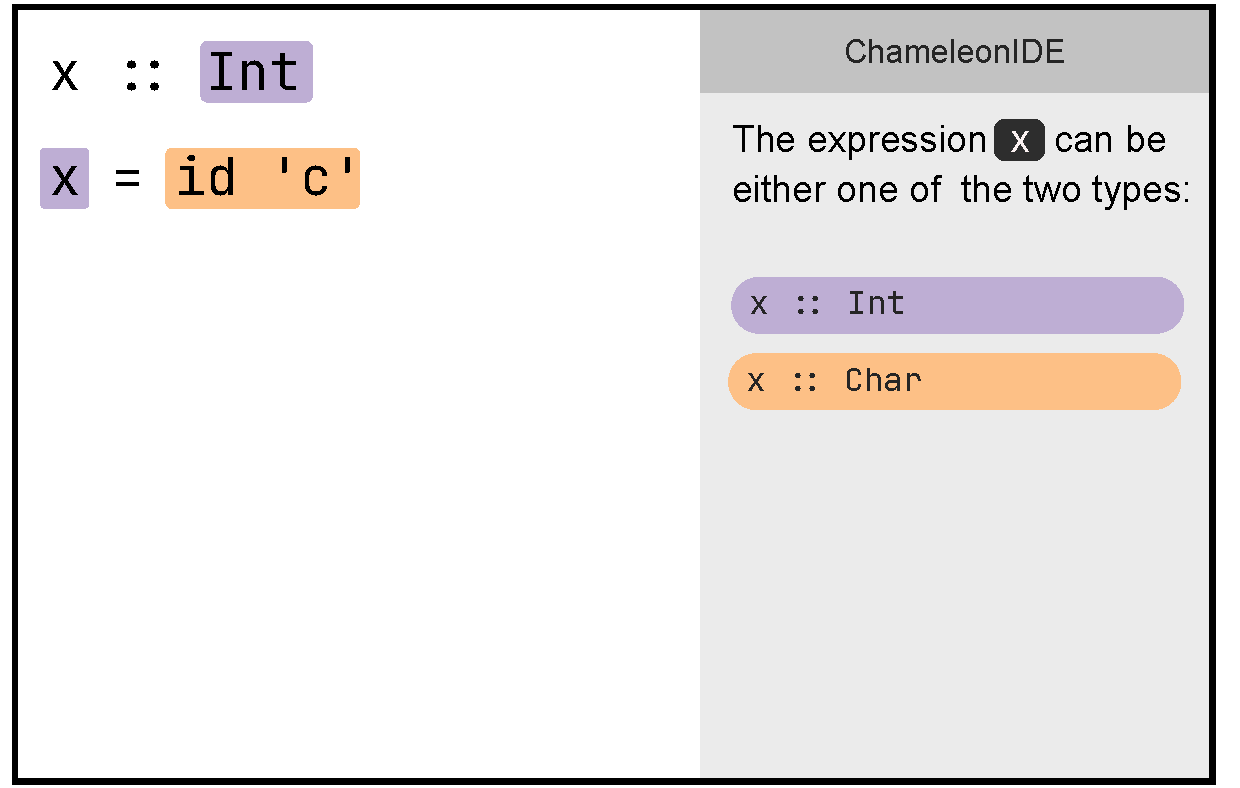
\includegraphics[width=\linewidth]{images/chameleon-v1.pdf}
%     \caption{
%         \chameleon{} 1
%         }
%     \label{fig:chameleon-v1}
% \end{figure}

Two  studies (1a \& 1b) were conducted to compare the effectiveness of solving type errors using \chameleon{} 1 and GHC compiler error messages. We choose GHC compiler error messages as the baseline because it is the canonical tool for working with type errors in Haskell. Although high-level tools like Haskell Language Server exist, they generally relay the GHC error messages verbatim. The procedure of these studies is shown in figure \ref{fig:procedure-1}.


Eight tasks were given in both studies. In study 1a, the tasks were taken from the exercises of the Haskell programming class in the authors' institute. These tasks cover a variety of type errors.  In the second study, the tasks are sourced from the top 20 Haskell topics on GitHub~\cite{github_github_2022}. The authors then manually added type errors into the program. In both studies, the type errors include simple mismatch, confusing syntax, missing instance, precedence and fixation, infinite types, and confusing list versus element. The categories of type errors to include in the tasks followed the common type errors in Tirronen's study \cite{tirronen_understanding_2015}. 

The  studies (1a \& 1b) are designed to answer the research question:
\begin{itemize}
    \item \textbf{RQ1.} Do programmers solve type errors faster with \chameleon{} than GHC compiler error messages?
\end{itemize}

\begin{figure}[h]
    \centering
    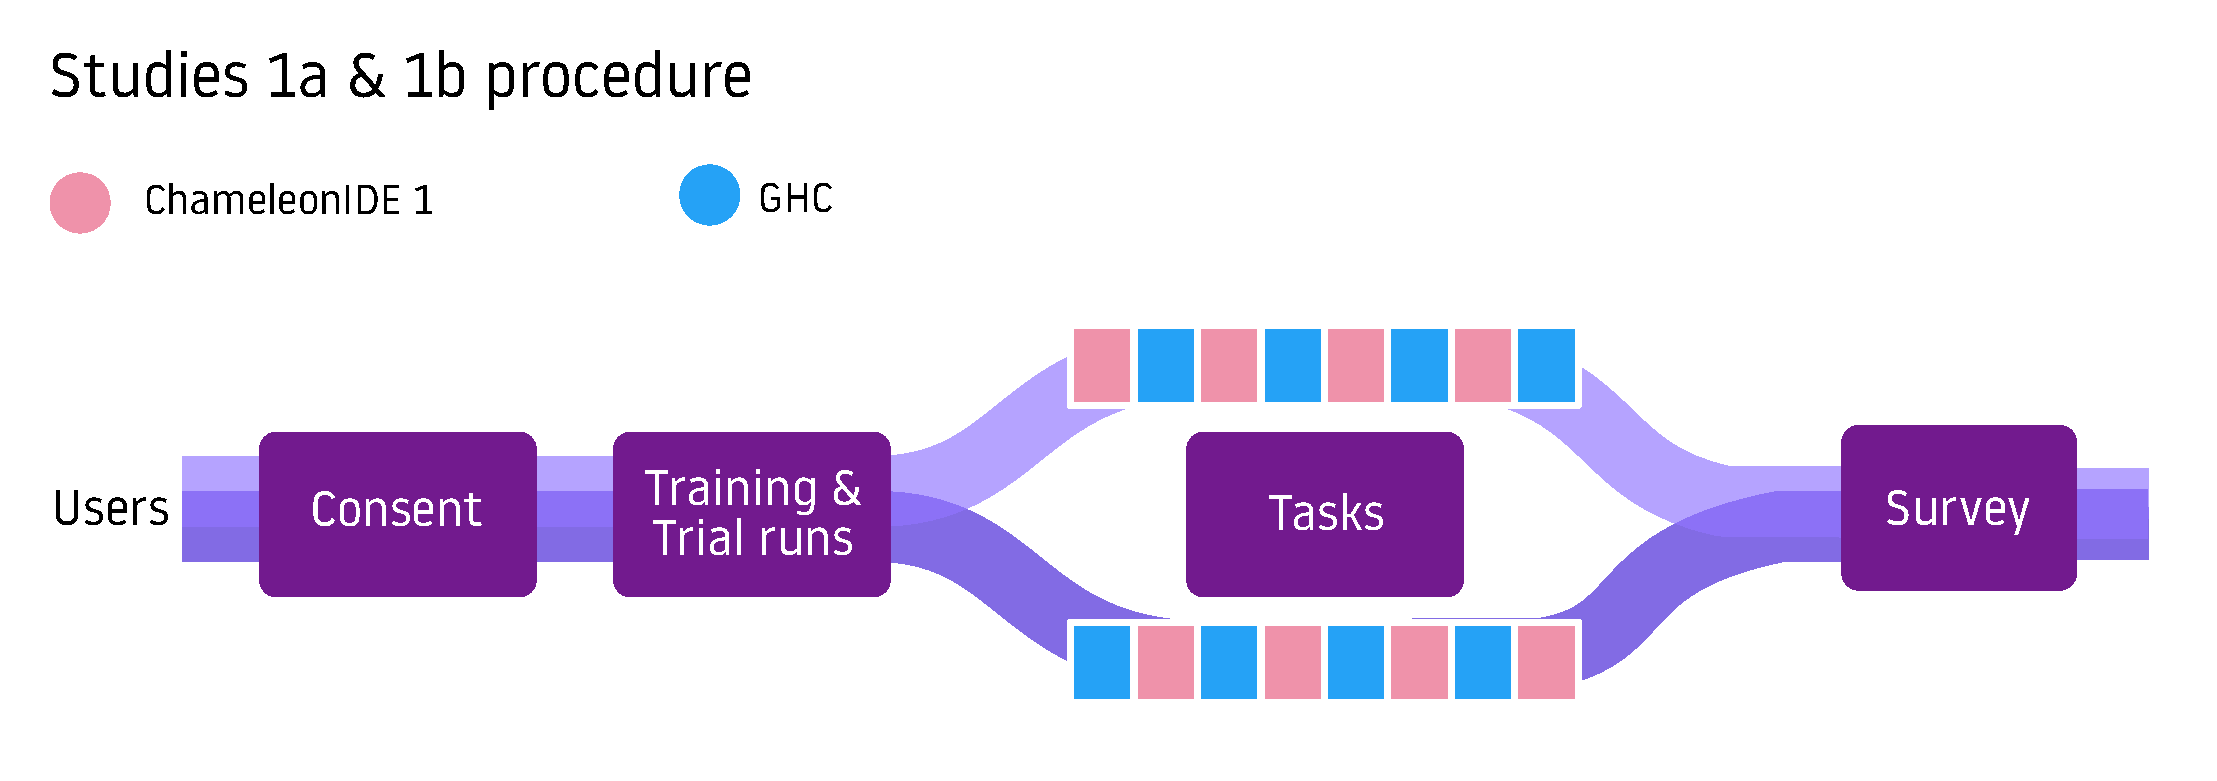
\includegraphics[width=\linewidth]{images/procedure-1.pdf}
    \caption{\todo{Does this figure really help at all?}}
    \label{fig:procedure-1}
\end{figure}

% The study investigates the effectiveness of \chameleon{} compared to the GHC compiler error messages. We chose GHC compiler error messages as it is the canonical tool for debugging type errors in Haskell. Although high-level tools like Haskell Language Server exist, they relay the GHC error message verbatim for type errors. Participants are asked to complete 8 tasks. The tool participants used during each task alternated between \chameleon{} and GHC. Task programs were sourced from HaskellWiki \cite{haskellwiki}. The author manually added type errors. The errors cover a range of common Haskell type errors, including abstract data types, wrong arity, control expressions (if and case), infinite types, and tuples. The lines of code (LoC) range from 7 to 17 (mean = 11, median=10.5).


% In total 39 participants finished the study. Among them, 12 participants have over five years of Haskell experience, and 5 participants have three or four years of Haskell experience. And 8 participants have one or two years of experience, and 5 participants used Haskell for under a year. The rest left the question unanswered.

\begin{figure}[h]
    \centering
    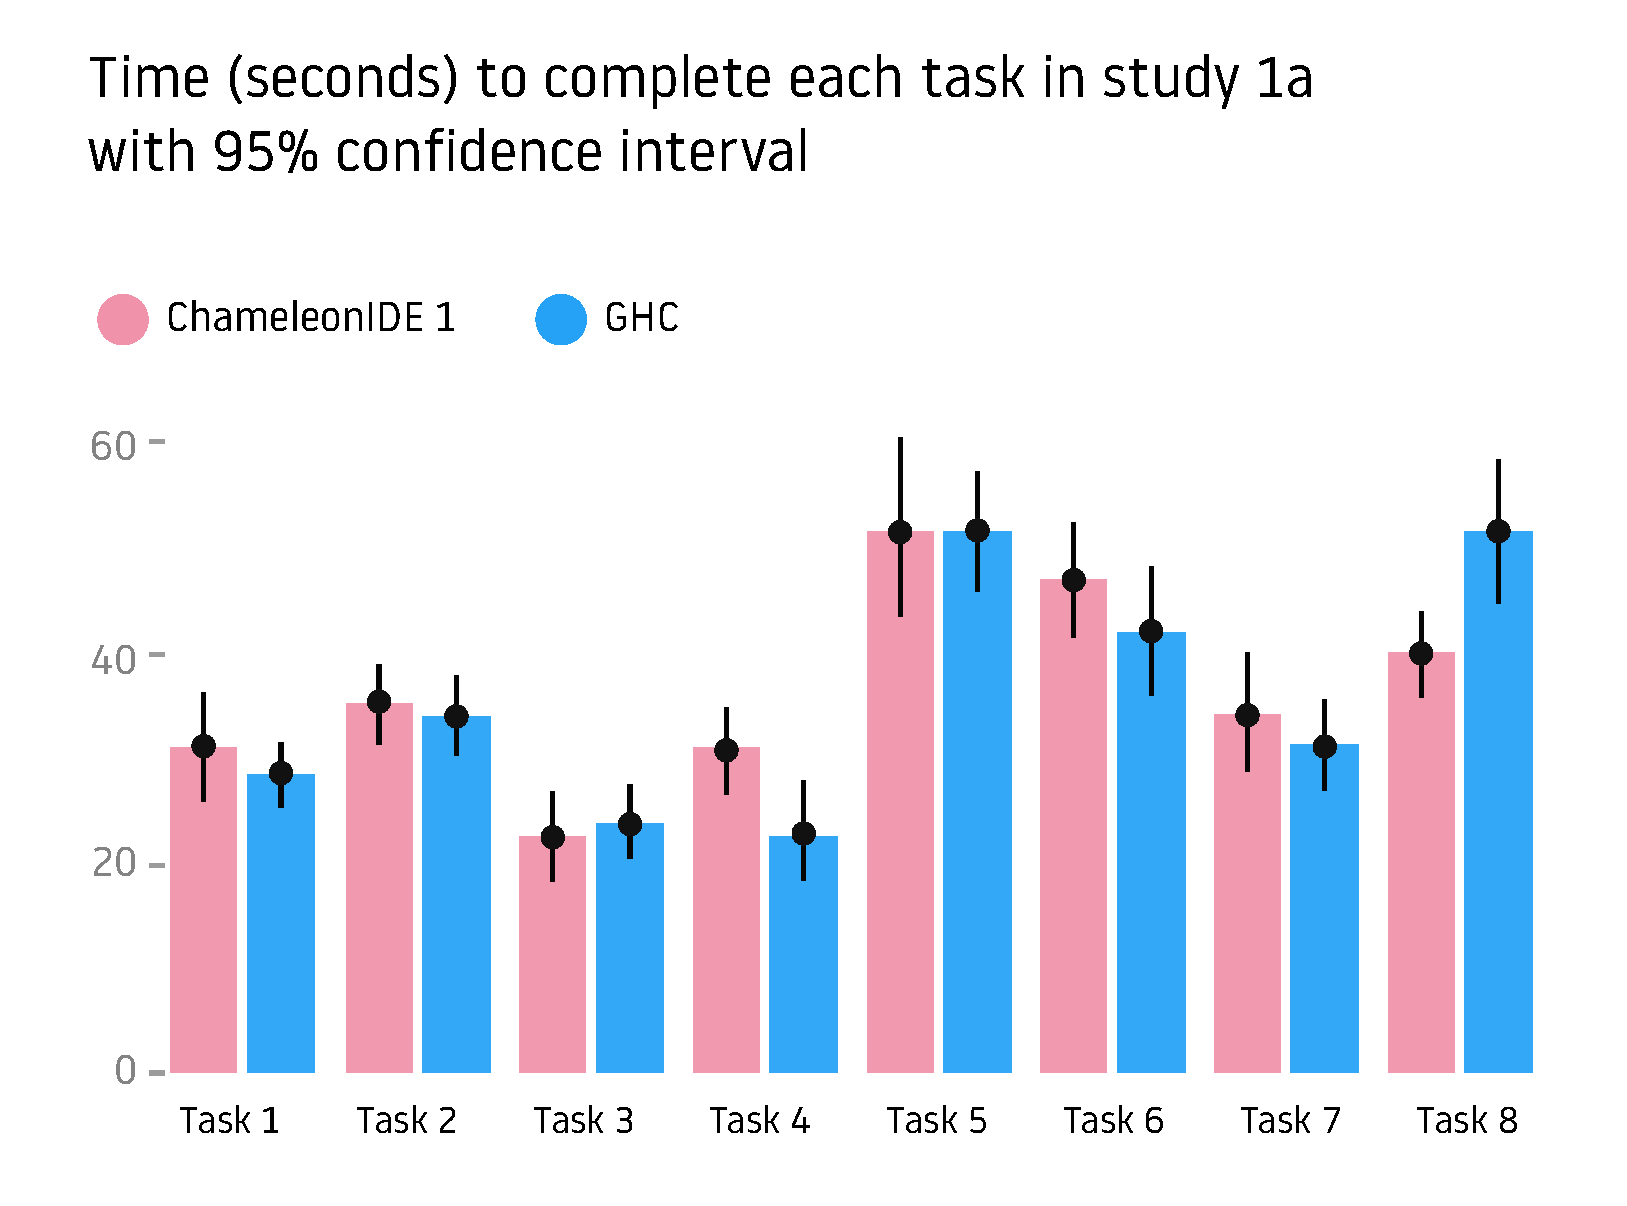
\includegraphics[width=\linewidth]{images/user-study-1a.pdf}
    \caption{Time to complete each task in user study 1a with 95\% confidence interval}
    \label{fig:analysis-1a}
\end{figure}


\begin{figure}[h]
    \centering
    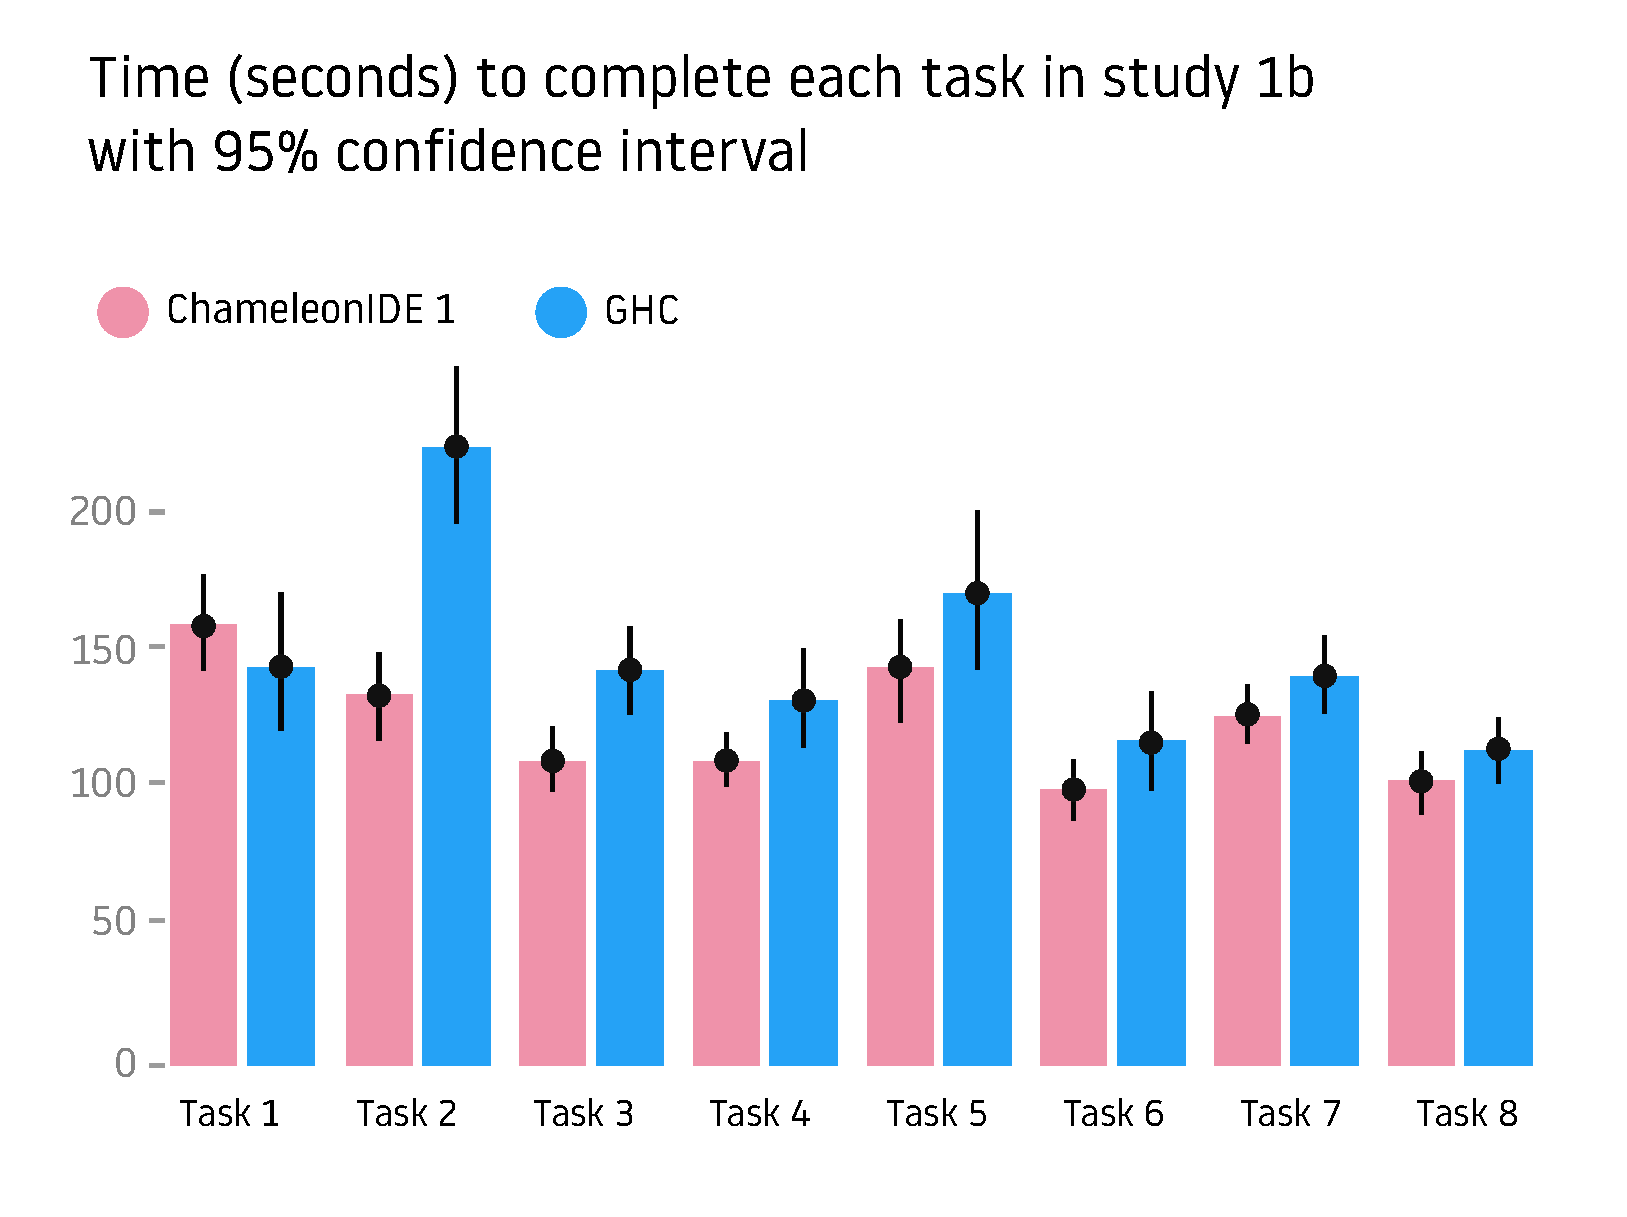
\includegraphics[width=\linewidth]{images/user-study-1b.pdf}
    \caption{Time to complete each task in user study 1b with 95\% confidence interval}
    \label{fig:analysis-1b}
\end{figure}

\subsubsection*{\textbf {Results}}

From the data collected during study 1a (\ref{fig:analysis-1a}), we were not able to identify which group performed better. For the trivial challenges we set for users, the individual differences are generally more significant than differences between treatments. One interesting observation is task 8, where the \chameleon{} group outperformed the GHC group more consistently (p-value = 0.002456, Wilcoxin signed test). The discrepancy is thought to be related to the nature of Task 8. It has a lengthier source file and involves more language features (abstract data types and high-level functions). GHC struggles to produce a relevant error message for this type of error. We hypothesized that we may observe a more significant difference using tasks with lengthier and more realistic source code. This hypothesis is also supported by the most common feedback (7 out of 35) the study 1a was that the tasks were too trivial to invite meaningful evaluation. One participant said, "Looks nicer than GHC, but without trying it on something more complicated, I cannot conclude whether it would help me in practice." 

In study 1b, the \chameleon{} group solved the type error faster (p =0.00742, Wilcoxin signed test) than the GHC group in almost all tasks (figure \ref{fig:analysis-1b}), barring task 1. For task 1, it is suspected that some participants spent more time exploring the interface of \chameleon{} due to its unfamiliarity and ineffective training. For all the other tasks, from the video recordings, we saw many \chameleon{} users confidently skip reading unrelated chunks of code, while GHC users generally read through the whole program. In harder problems and messier code, we notice programmers start to report the benefits of \chameleon{}. "It's most useful feature that I noticed was that it points out the locations of both conflicting uses; GHC often makes it difficult to figure out how it's coming to a conclusion about a type." reported one participant. "I think \chameleon{}  does a much better job than GHC's error messages. I like that it shows the sources for the type judgments. This makes it quite easy to figure out how to rectify errors." reported another participant.

% \begin{itemize}
%     \item {It has a longer source file than other tasks (only shorter than task 6, but task
%     6 contains two independent type errors while task 8 is one connected task
%     error);}
%     \item {It is more complex than others (involves abstract data types and function application); and
%     }
%     \item {
%         GHC struggles to produce a relevant error message for this type of error.
%     }
%   \end{itemize}


  

% \begin{figure}[H]
%     \centering
%     \Description{A screenshot from user study 1}
%     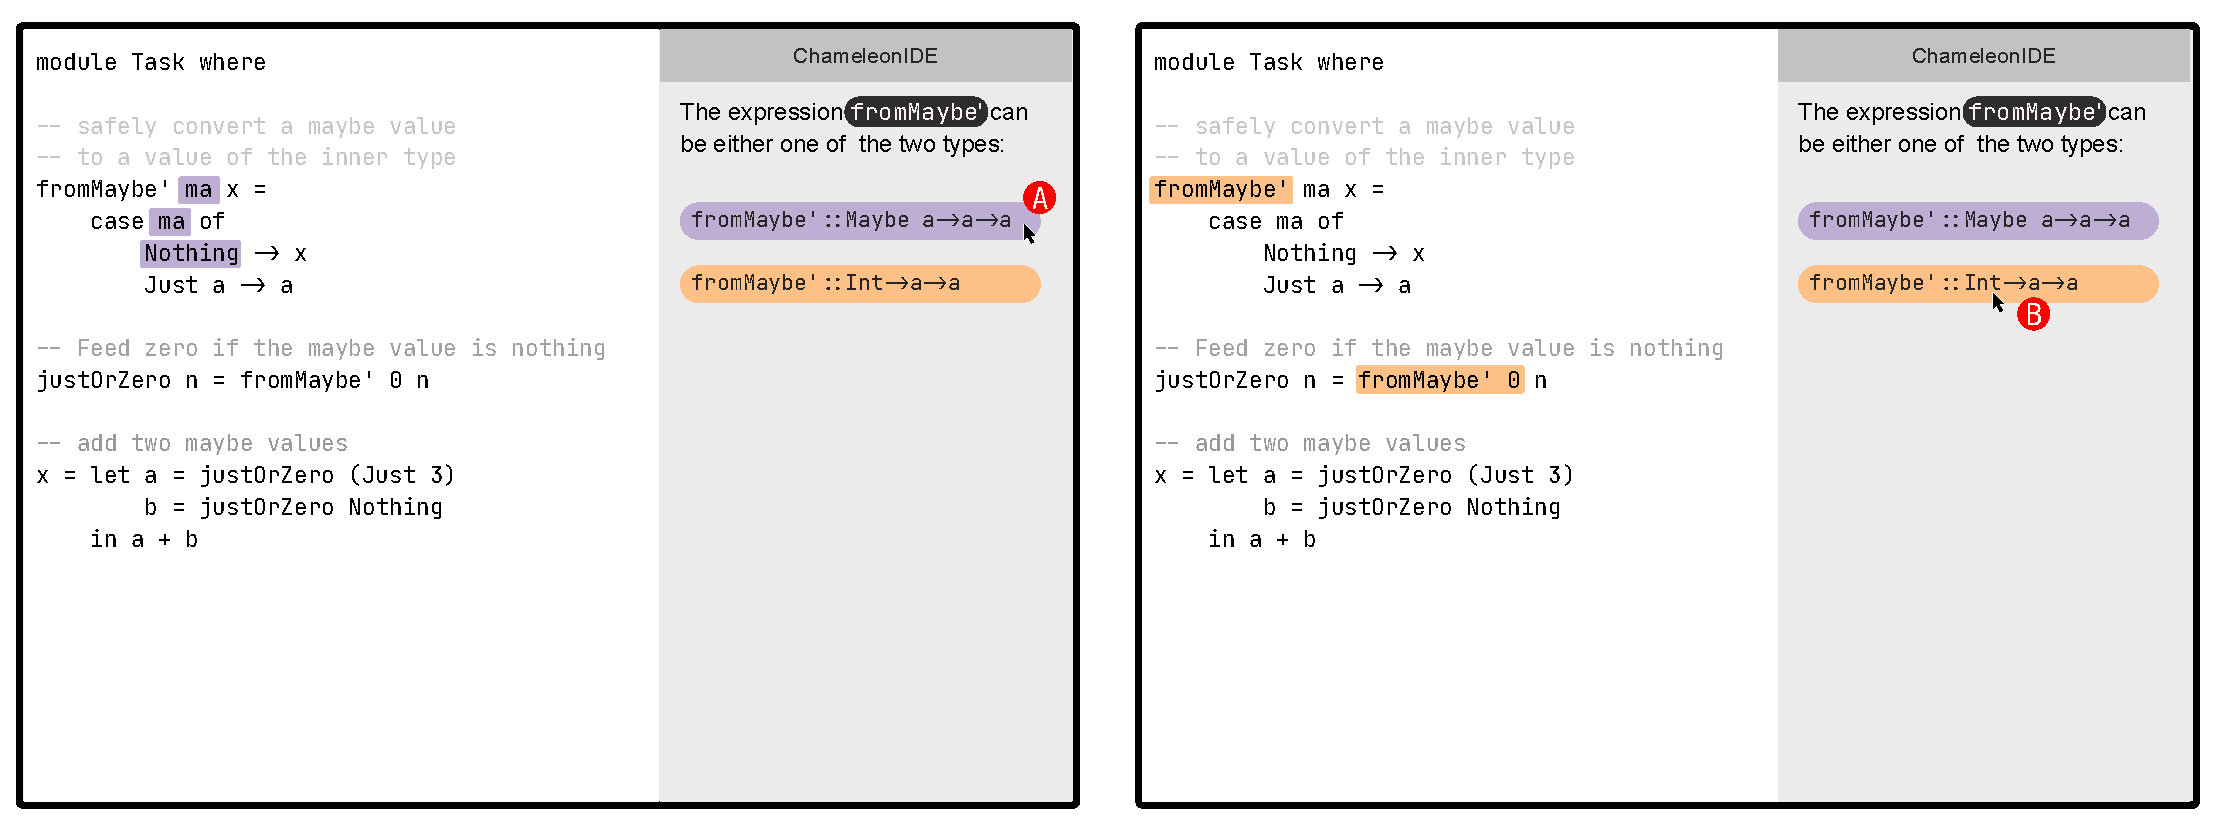
\includegraphics[width=\textwidth]{round1-screenshot.pdf}
%     \caption{
% One participant working with \chameleon{}  managed to identify the most probable location of the error (the application of `fromMaybe'` on line 11) by hovering over the two alternative types. The participant then quickly realized that the first argument `0` (highlighted in orange) is inconsistent with the definition where it is case matched to a `Nothing` value (highlighted in purple). After two retries with short hesitation the participant found the correct fix (by reversing the order of `0` and `n`).
%     }
%     \label{fig:r1-task8}
% \end{figure}


% \begin{figure}[htb]
%     \centering
%     \Description{A screenshot from user study 1}
%     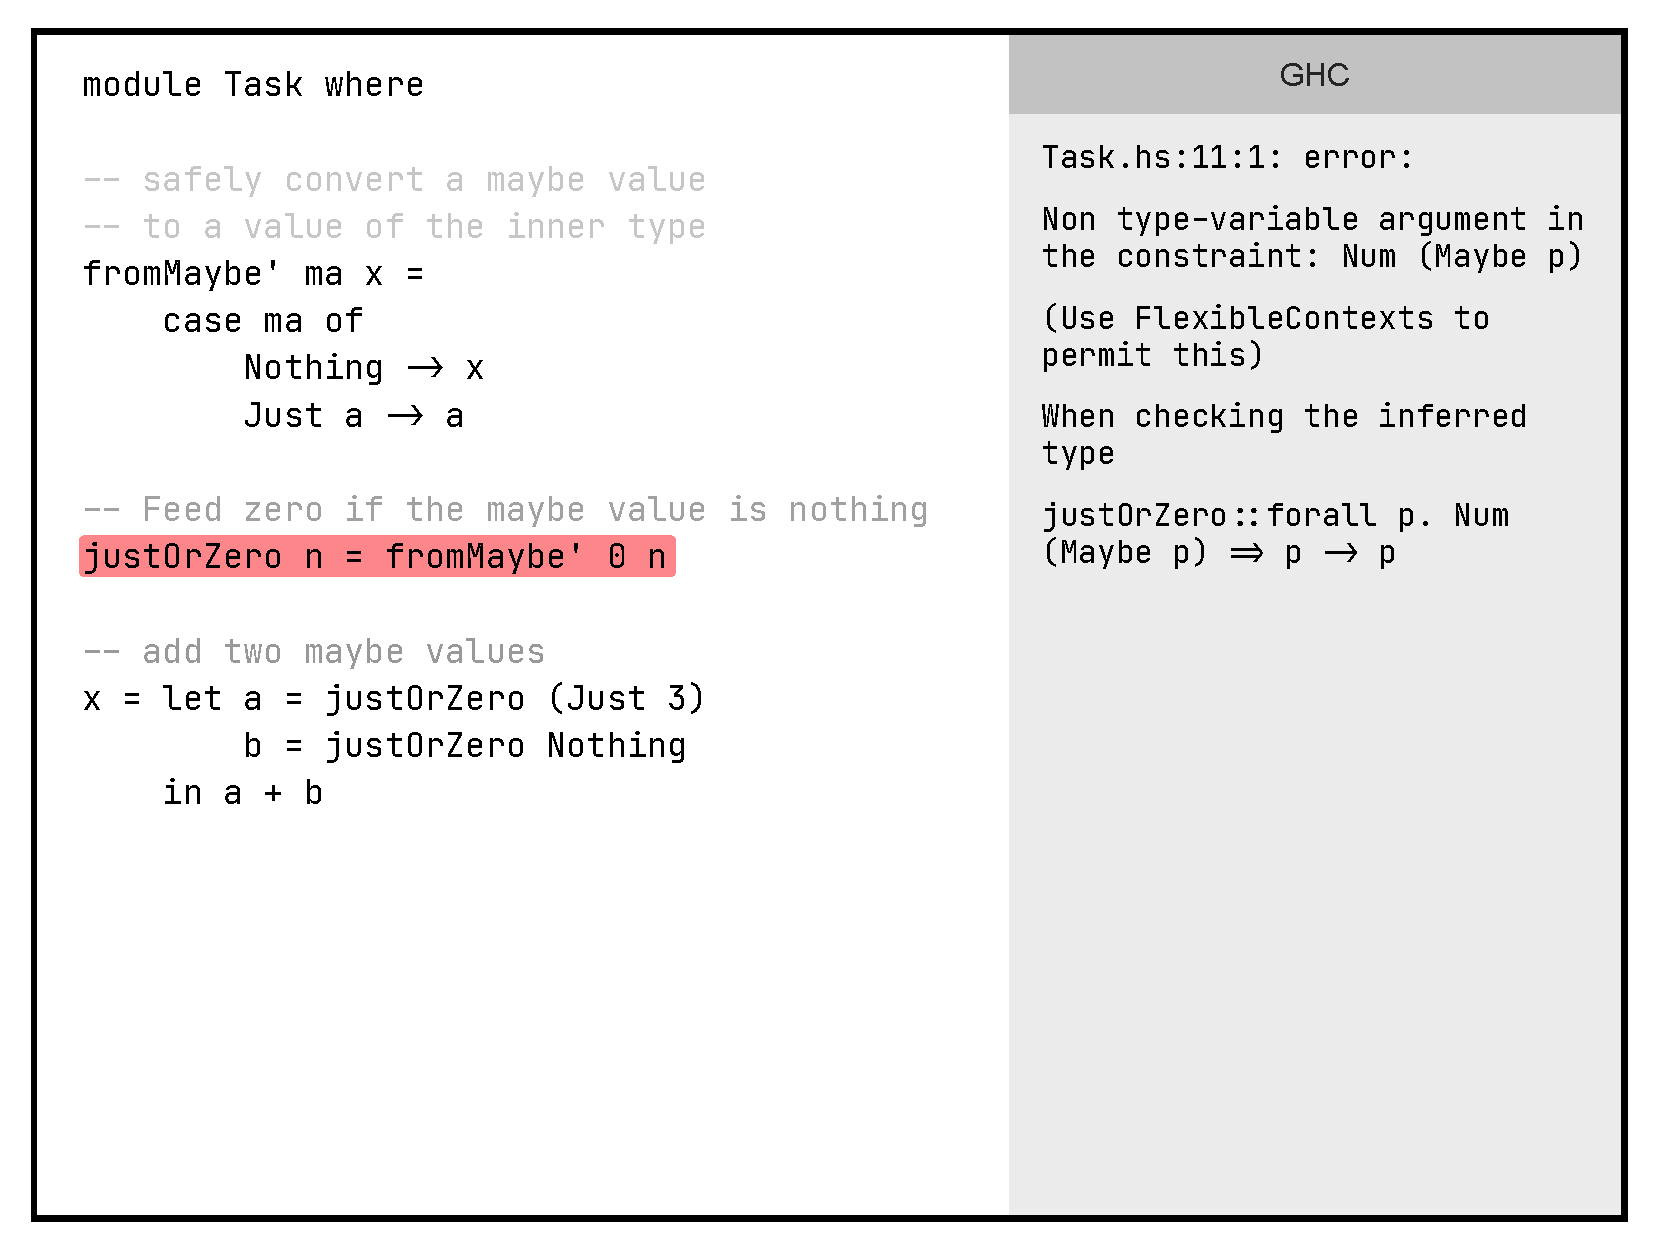
\includegraphics[width=\textwidth]{round1-screenshot-ghc.pdf}
%     \caption{
%         In task 8, participants using GHC took longer pauses at this task before committing to further investigation, either carefully reading the whole text or figuring out the meaning of the error message. The GHC error message is unfortunately unhelpful for this task.
%     }
%     \label{fig:task8-ghc}
% \end{figure}




\subsubsection{\textbf{\chameleon{} 2}}  \label{sub:us4}

\chameleon{} 2 is latest version of \chameleon{}. Advanced debugging features such as deduction steps and candidate expressions were available in this iteration. In addition, mode switching is enabled by default as well. A few other user interfaces were designed and prototyped between the development of \chameleon{} 1 and \chameleon{} 2. Study 2 was designed to evaluate \chameleon{} 2.  We were trying to answer the research question: \textit{How do programmers use the interactive features in \chameleon{} 2?}. More specifically, we were trying to inquiry the following three sub-questions:
\begin{itemize}
    \item Do programmers prefer switching modes during debugging type errors?
    \item What are programmers' preferences among the three modes provided by \chameleon{} 2?
    \item How do programmers use the advanced features provided by \chameleon{} 2?

\end{itemize}

During the study, the initial mode of each task alternated through the three different modes and repeated three cycles in nine tasks. The order of the three modes in each cycle is counterbalanced among all participants. However, participants can switch to other modes at any time (figure \ref{fig:procedure-2}). 



\begin{figure}[h]
    \centering
    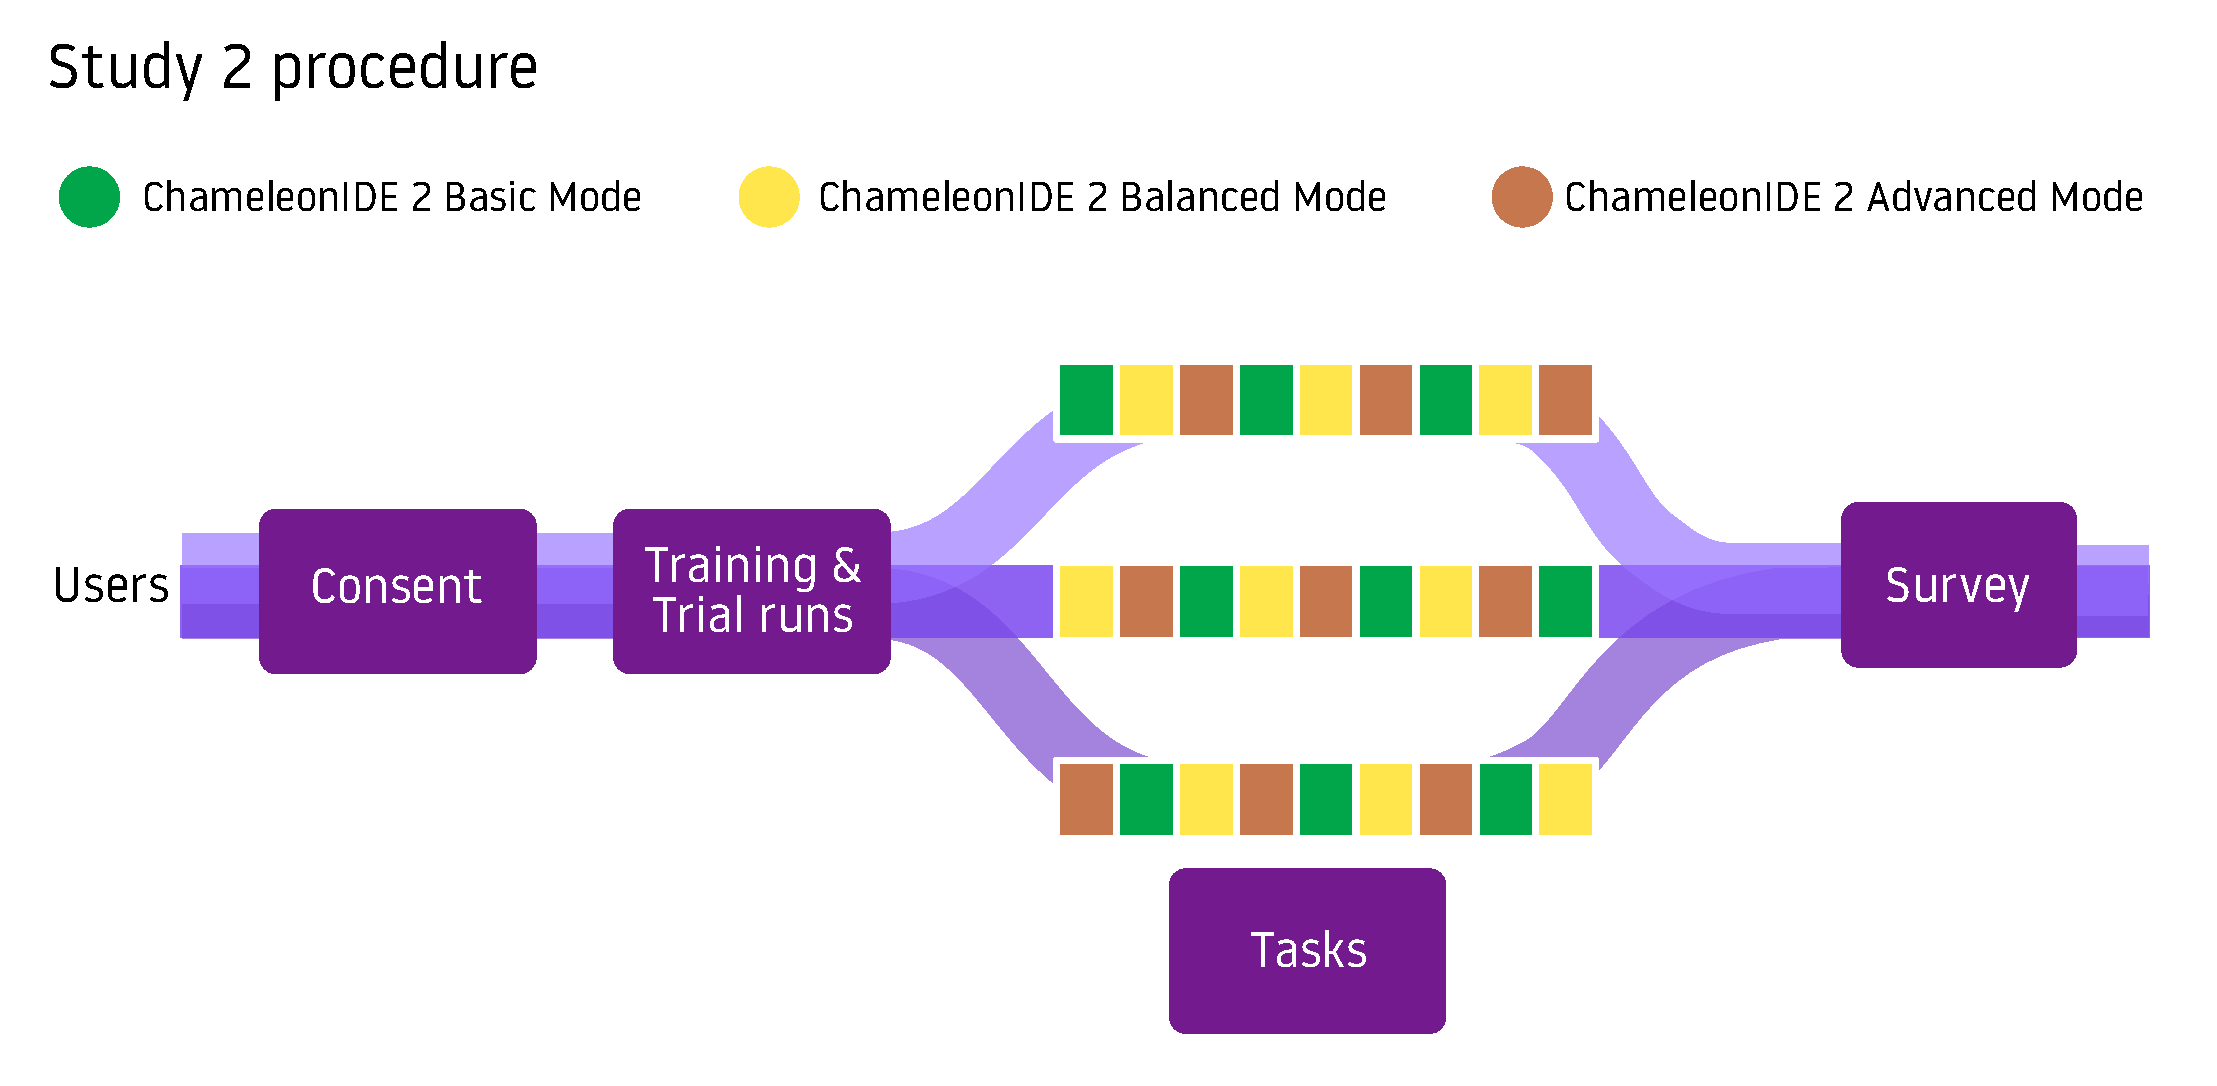
\includegraphics[width=\linewidth]{images/procedure-2.pdf}
    \caption{\todo{Does this figure really help at all?}}
    \label{fig:procedure-2}
\end{figure}

\subsubsection*{\textbf{Results}} 

The study of \chameleon{} 2 is an exploratory study. We were expecting to let programmers discover their own way of using the tool. In post hoc analysis of the collected log data, we were able to extrapolate some interesting patterns of how the tool was used. We share a few of our observations in this section.


The most striking feature of the data is users' tendencies to use the tool differ wildly. Some users used the feature extensively however some users completed the tasks without actively exploring the given information. Based on this discrepancy, we divided the users into three groups.

\begin{tabularx}{\linewidth}{ 
  | >{\raggedright\arraybackslash}X 
  | >{\raggedright\arraybackslash}X  | }

    \hline
        Interaction level & Description \\ \hline
        Minimal Interaction & Users completed the tasks by making changes in source code, type checking, and reading error messages. \\ \hline
        Low Interaction & Users only actively used universal features in all modes, for example, hovering on "Possible type 1" and "Possible type 2" to narrow down error space. \\ \hline
        High Interaction & Users did everything from the Common feature group but used features specific to the Balanced mode and the Advanced mode, such as activating steps and expression cards. \\ \hline
\end{tabularx}


As shown in  figure \ref{fig:r4-analysis}, the time to complete each task roughly relates to the interaction level of participants. Participants with higher interaction levels generally performed better in the tasks, and the lowest level was worse (one-way ANOVA since we have three samples, p = 0.0368). The results from three tasks stand out from the general trend: in Tasks 4 and 6, higher interaction users performed worse, and in task 9, the general trend is exaggerated. As discussed in user studies 1 and 2, it is likely related to the nature of these tasks. Tasks 4 and 6 are shorter than other tasks. The ideal fixes for these two tasks are placed relatively early in the source code (both in the first two lines of the source code). These may be useful because following the natural reading order will allow participants to skip lines on the bottom, and thus the advantage of \chameleon{} is less critical. On the other hand, task 9 is the lengthiest task of all. It also involves more complex features, such as mutually recursive type definitions.

\begin{figure}[h]
    \centering
    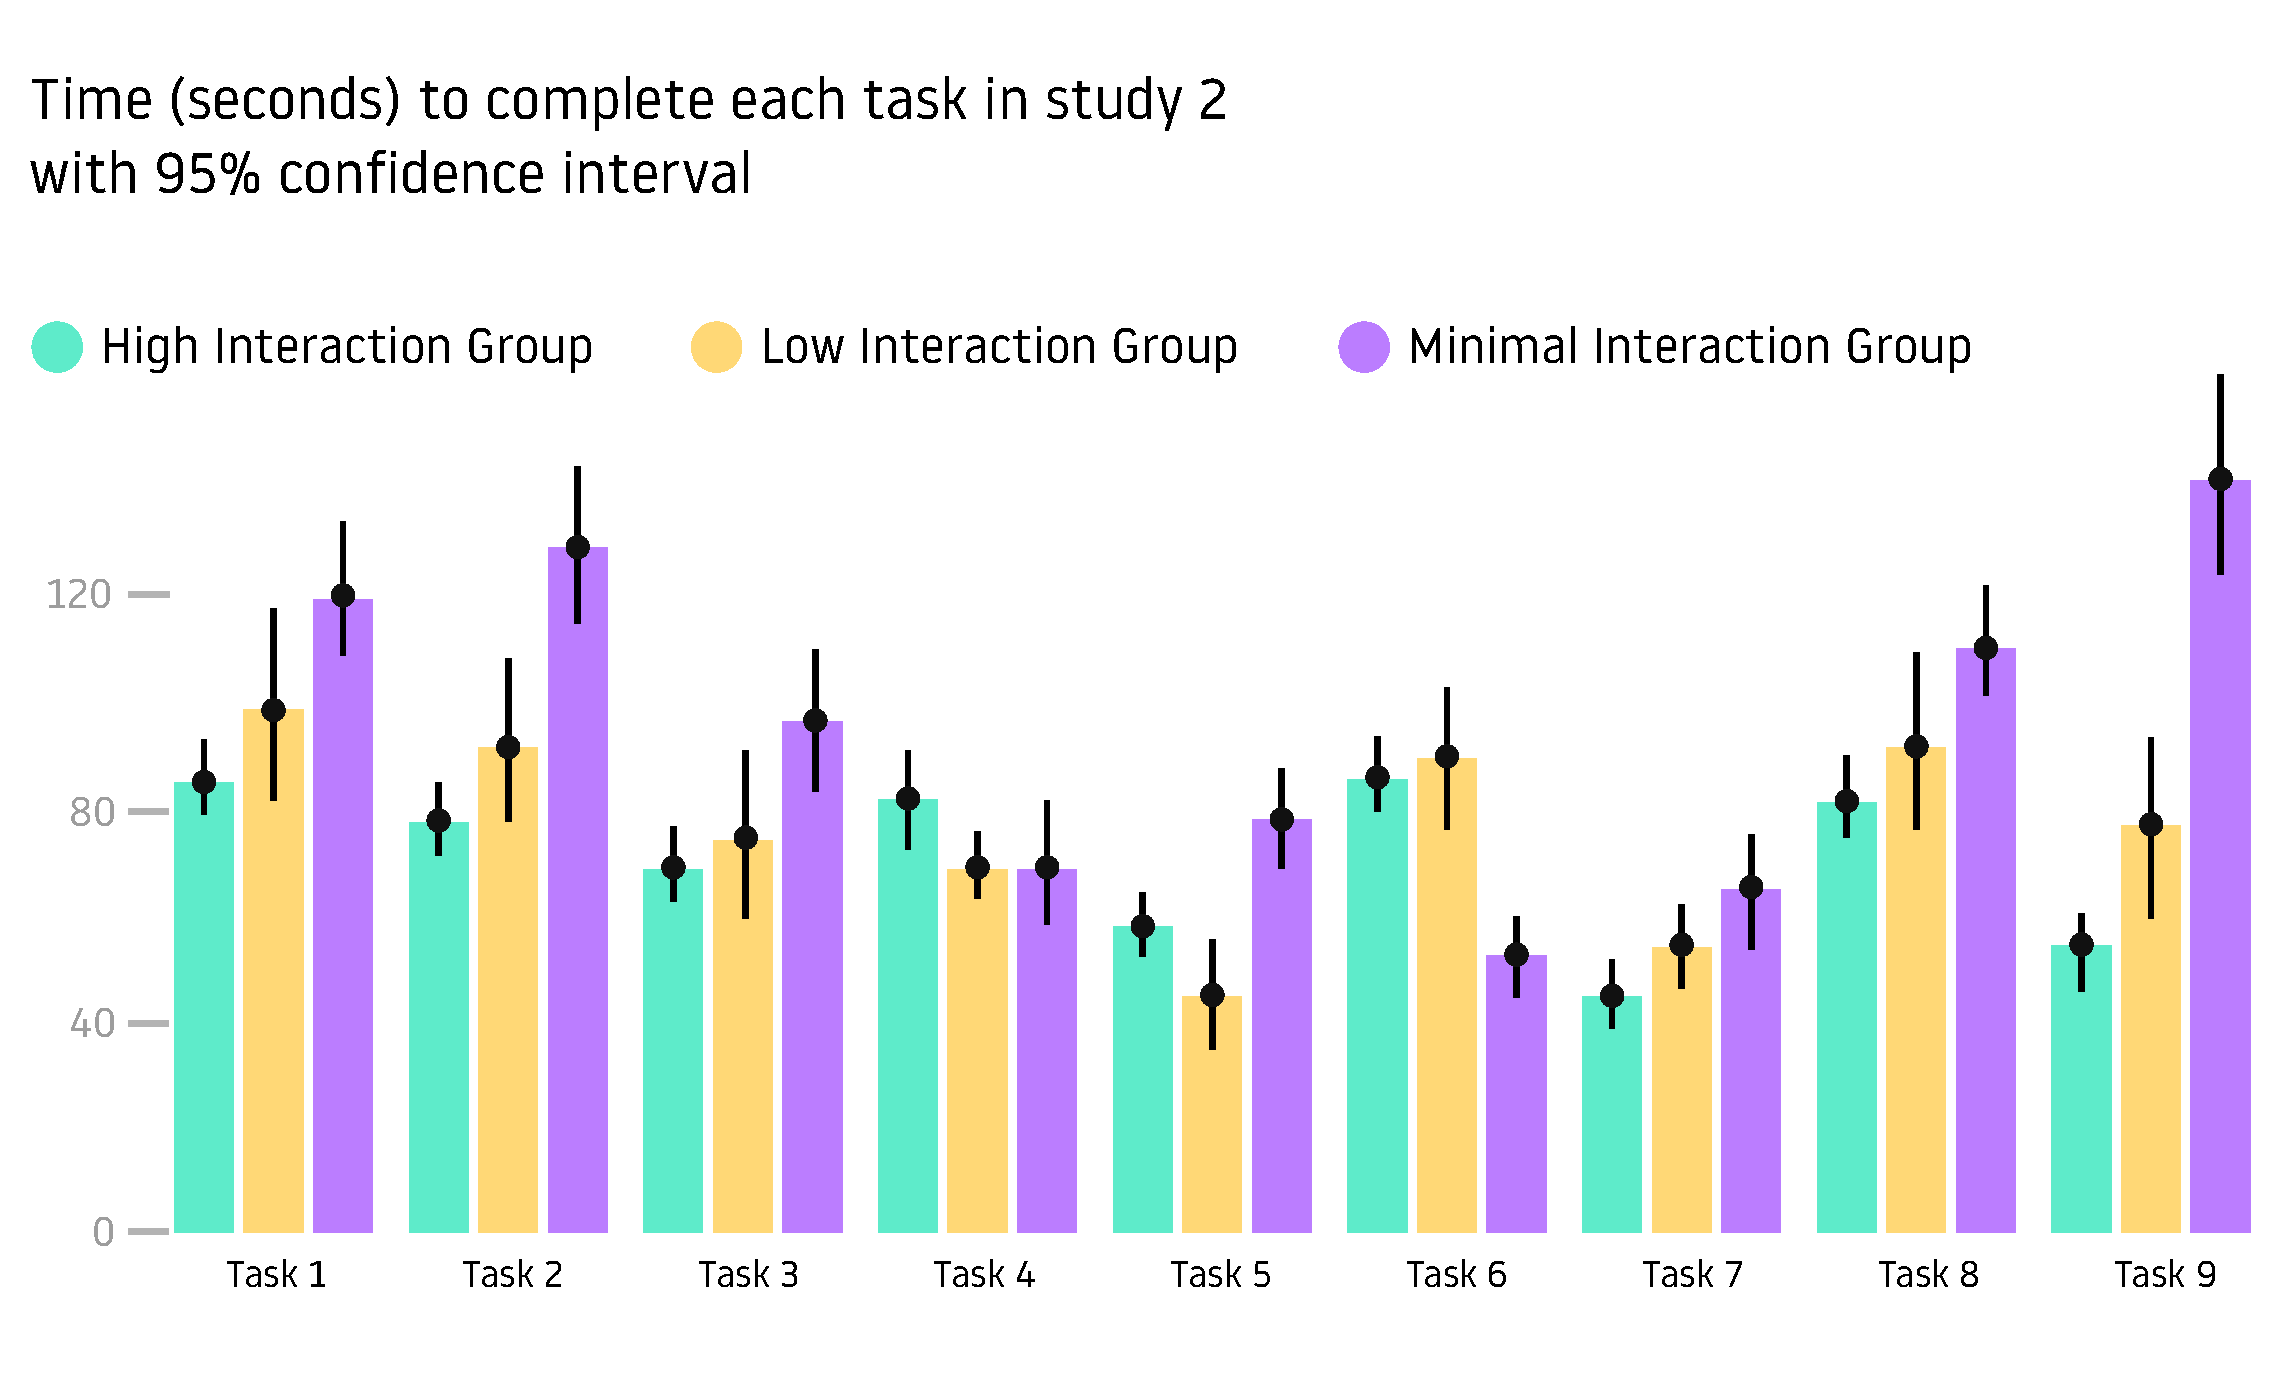
\includegraphics[width=\linewidth]{images/user-study-2.pdf}
    \caption{Time to complete each task in study 2 with 95\% confidence interval}
    \label{fig:r4-analysis}
\end{figure}


% \begin{figure}[h]
%     \centering
%     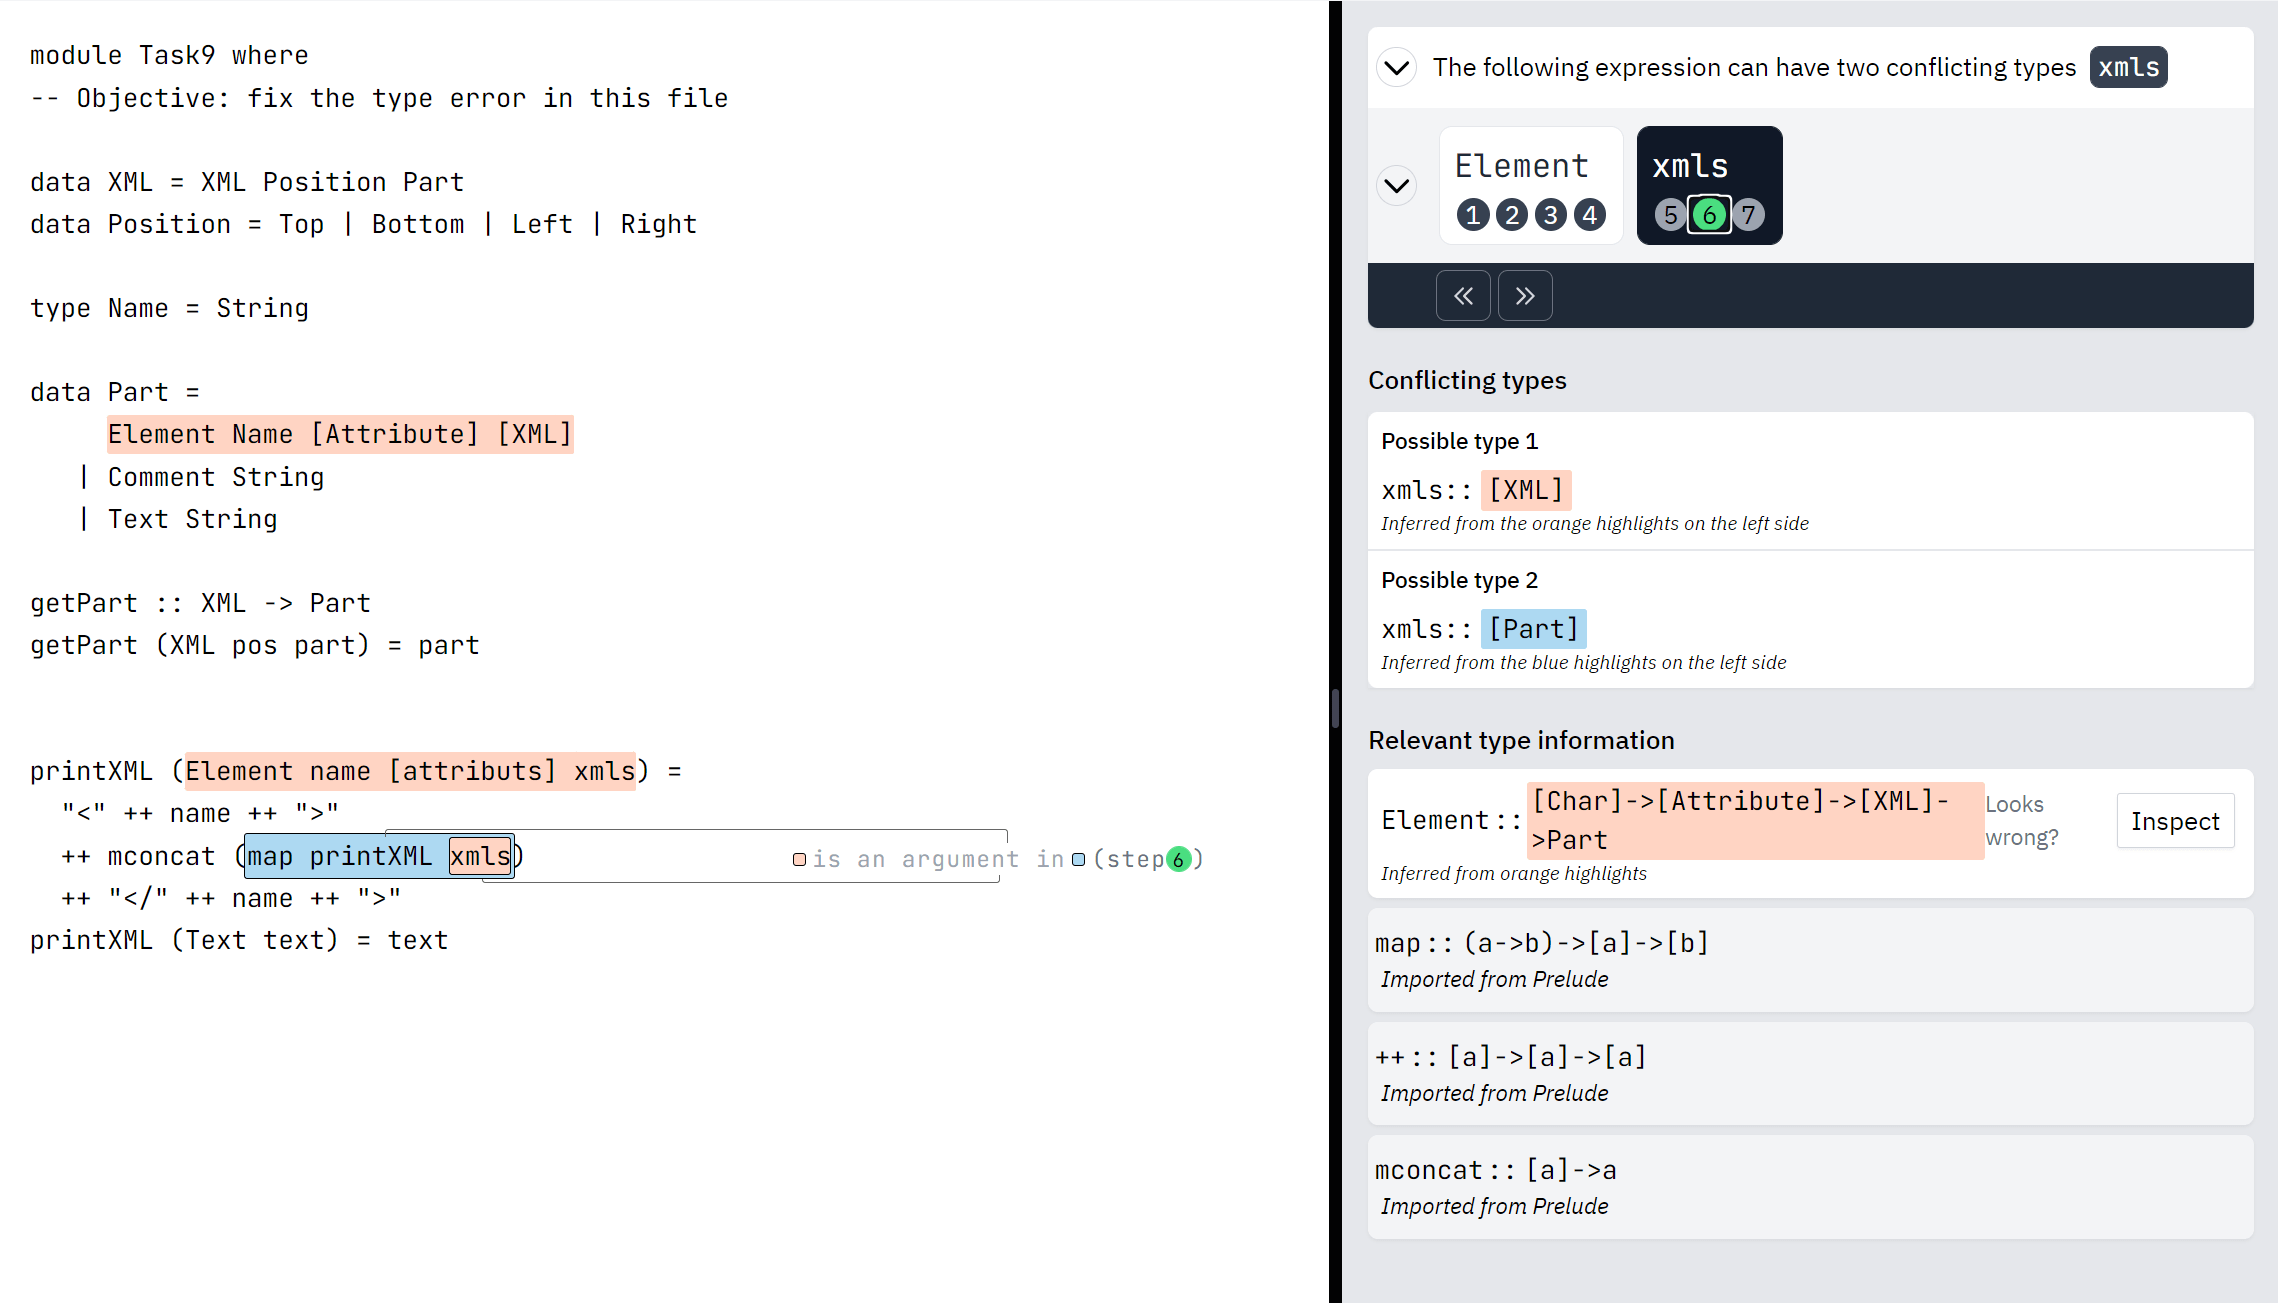
\includegraphics[width=\linewidth]{images/r4-task9.png}
%     \caption{
% High interaction users were able to locate the exact line for a potential fix after navigating to deduction step 6 or 7, which directly revealed the true cause of the type error. After this, 12 out of 15 high interaction users provided the most ideal fix in the first try. Low interaction group  takes longer time to examine the problem, provided wrong fixes in the initial trials. One participant fixed a minor run-time issue (a problematic pattern matching of `[attributes]` on line 18) however failed to identify the culprit of the type error. This location is not pinpointed by \chameleon{} and therefore it is understandable that programmers who used the deduction steps would be able to ignore this part of the source code.
%     }
%     \label{fig:r4-task9}
% \end{figure}


Another observation is when using the mode switching feature of \chameleon{}, we find presenting the starting mode and finishing mode of each task and each participant in a confusion matrix is very telling (Fig. \ref{fig:r4-mode-switching}). 
This observation suggests two characteristics of using multi-mode debugging tools. First, programmers are generally reluctant to switch modes (146/277 changing modes vs. 131/277 staying in the same mode). Second, when changing modes, programmers generally switch to the more informative modes instead of, the more concise ones.
\begin{figure}[h]
    \centering
    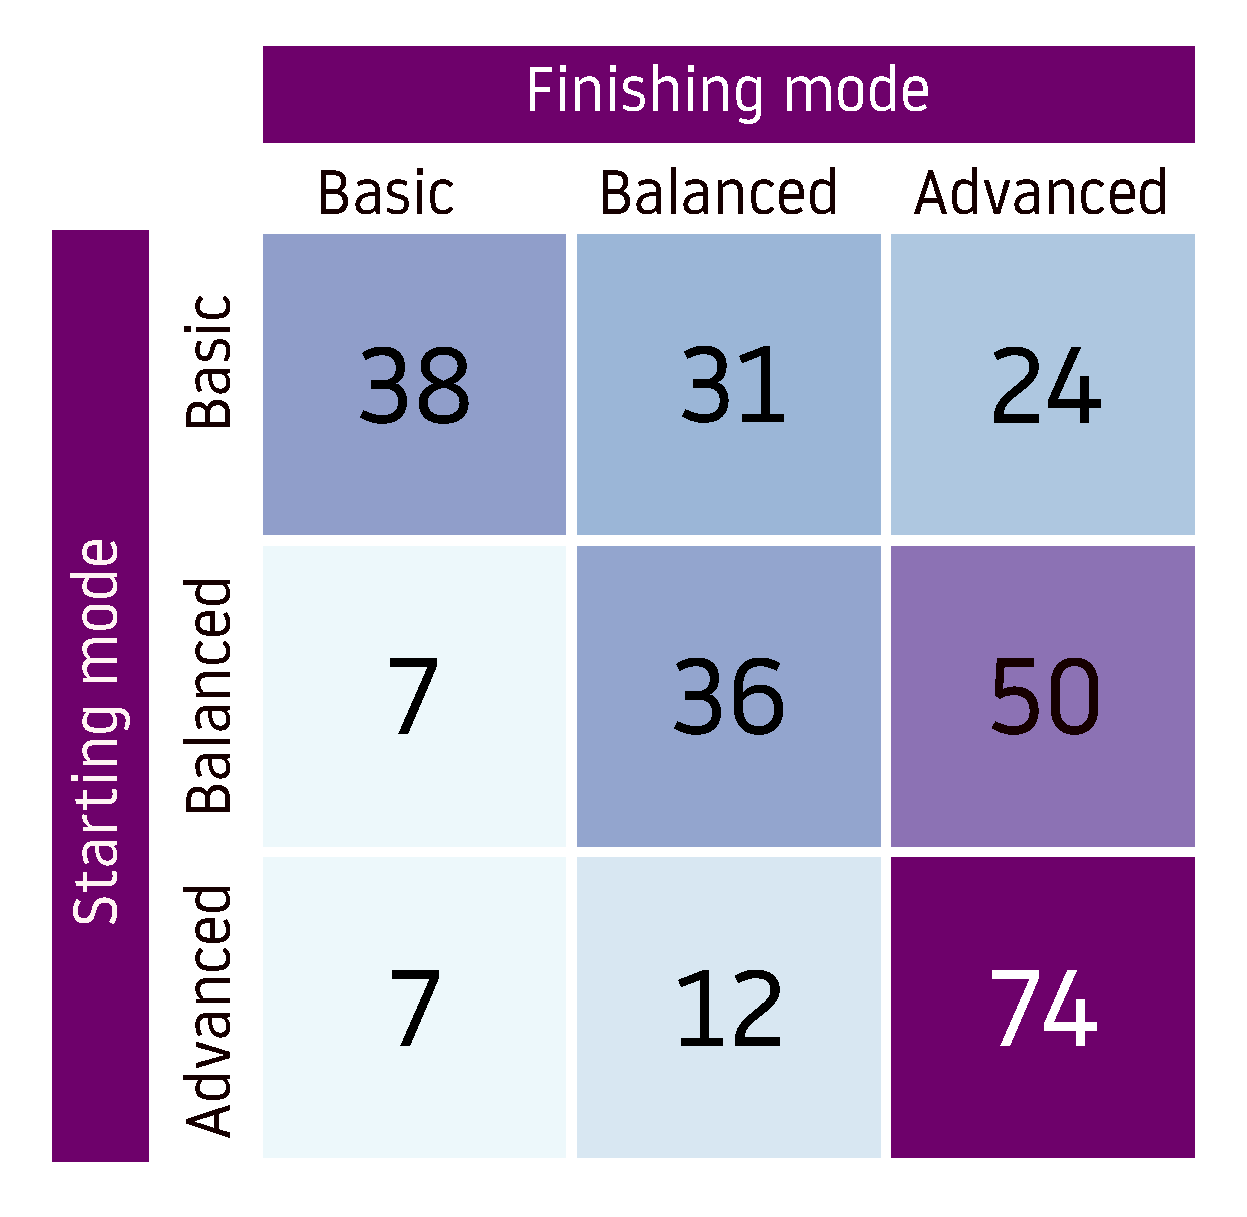
\includegraphics[width=\linewidth]{images/mode-switching.pdf}
    \caption{
        % The rows represent the finishing mode, columns starting modes.
    }
    \label{fig:r4-mode-switching}
\end{figure}


